
\section{\textcolor{black}{Uncertainty}} % Sections are added in order to organize your presentation into discrete blocks, all sections and subsections are automatically output to the table of contents as an overview of the talk but NOT output in the presentation as separate slides

%------------------------------------------------


\begin{frame}
	\frametitle{Real world with uncertainties}
\begin{columns}
    \column{0.5\textwidth}
    \begin{figure}
    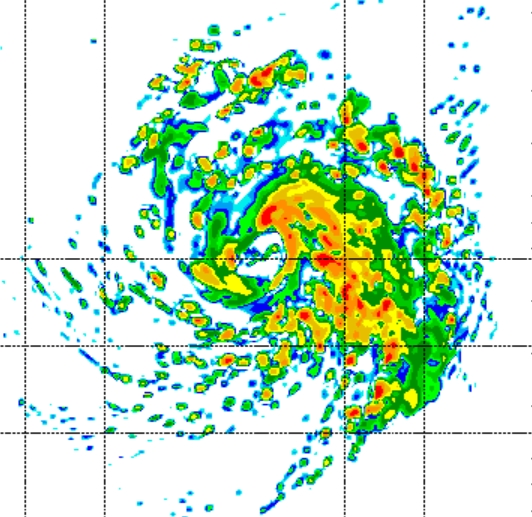
\includegraphics[width = 6cm]{figures/figure-typhoon.png}     
    \end{figure}    \footnotetext{\href{https://en.wikipedia.org/wiki/Weather_Research_and_Forecasting_Model}{Source: Wikipedia}}
    \column{0.5\textwidth} 
    \begin{figure}
    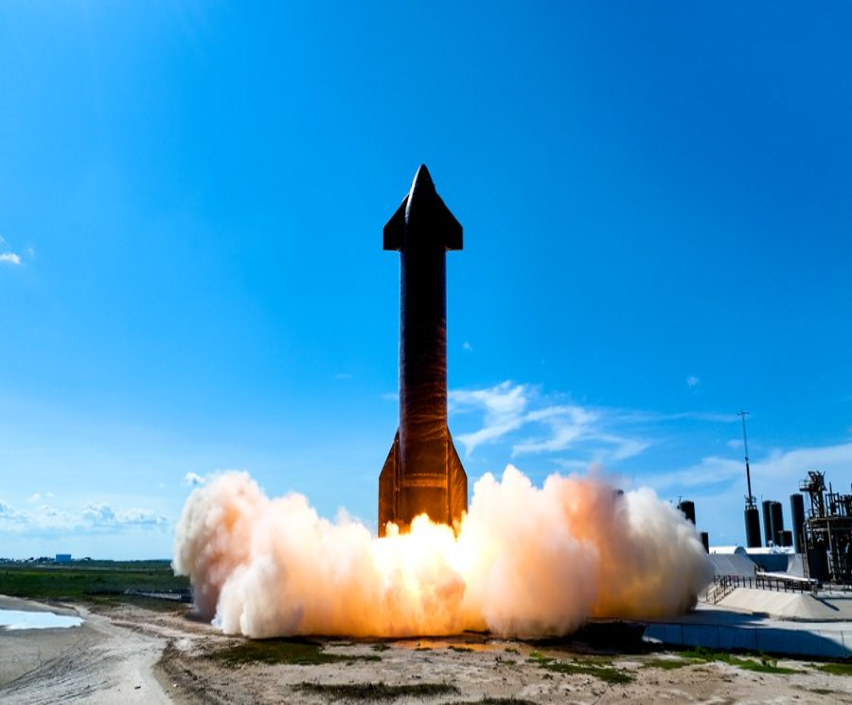
\includegraphics[width = 7.2cm]{figures/figure-rocket.pdf}   
    \end{figure}    
\end{columns}
\end{frame}

%------------------------------------------------
\begin{frame}
\frametitle{Types of two uncertainties}
\framesubtitle{Aleatoric vs epistemic}

\begin{columns}
    \column{0.7\textwidth}
        \begin{figure}
        \centering
            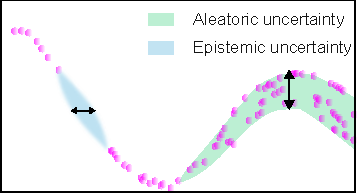
\includegraphics[width = 9cm]{figures/aleatoricvsepisidemic.pdf}
            \caption{Aleatoric uncertainty vs Epistemic uncertainty}
        \end{figure} 
    \column{0.3\textwidth}
     \textbf{Distinguish}:
     \begin{block}{Aleatoric uncertainty}
statistical variability, inherently random effects (\textbf{irreducible})
     \end{block}
     \begin{block}{Epistemic uncertainty}
model uncertainty, a lack of knowledge (\textbf{reducible})
     \end{block}    
    \end{columns}
\end{frame}
%--------------------------------

\begin{frame}
\frametitle{Two examples: aleatoric or epistemic?}
\begin{columns}
    \column{0.4\textwidth}
    \begin{example}{Gambling}
        \begin{itemize}
            \item what if guess the number of the dice
            \item what if guess the mass of the dice
        \end{itemize}
    \end{example}
    \column{0.4\textwidth}
    \begin{example}{Seeing doctors}
        \begin{itemize}
            \item what if a patient's symptoms vary from day to day
            \item what if the diagnostic technique is not advanced enough
        \end{itemize}
    \end{example}
\end{columns}


\end{frame}
%----------------------------------------------------------


% \begin{frame}
% \frametitle{Type two: epistemic uncertainty}
%     \begin{columns}[]       
        
%     \column{0.5\textwidth}  
%         \centering

%         \begin{figure}
%             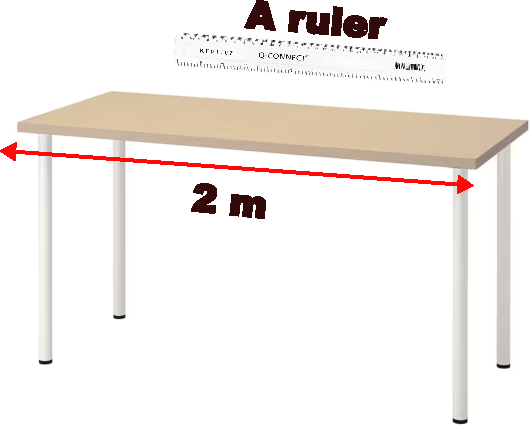
\includegraphics[scale=0.8]{figures/figure-table_ruler.pdf}
%         \end{figure}
 
      

%     \column{0.5\textwidth}
   
     
%     \textbf{Random variables: }

%     $x_{i} = x^{\star} (\text{2m}) \pm \epsilon$, $\epsilon \sim \mathcal{N}(0,\sigma^2)$

%     $ x_{i} \sim iid$

%     $\boldsymbol{x} = (x_1,x_2,\cdots,x_n)$
%     \bigskip
    
%    \textbf{mean:} 

%    \begin{equation}
%    \begin{aligned}
%       \mathbb{E}(\boldsymbol{x}) &= \frac{1}{n} \sum_{i=1}^{n} x_i \\
%        &= \mathbb{E}(x^{\star}) (\text{2m}) +\mathbb{E}(\boldsymbol{\epsilon})\\  
%    \end{aligned}
%    \end{equation} 

% When $n \rightarrow \infty$, $\mathbb{E}(\boldsymbol{x}) \approx x^{\star} + 0 \approx$ 2 (m)

% \end{columns}
% \end{frame}

%----------------------------------------------------------


\begin{frame}
\frametitle{Uncertainty components:}
\Large\textbf{Total uncertainty $\approx$ aleatoric uncertainty $+$ epistemic uncertainty}
\begin{figure}
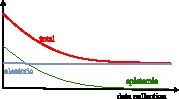
\includegraphics[scale=2.5]{figures/figure-total_Uncertainty.pdf}
\end{figure}

\end{frame}
%----------------------------------------------------------
\begin{frame}
\frametitle{Not simple as it is}
\framesubtitle{Mix of aleatoric and epistemic: Involve too much subjectivity}
\begin{figure}
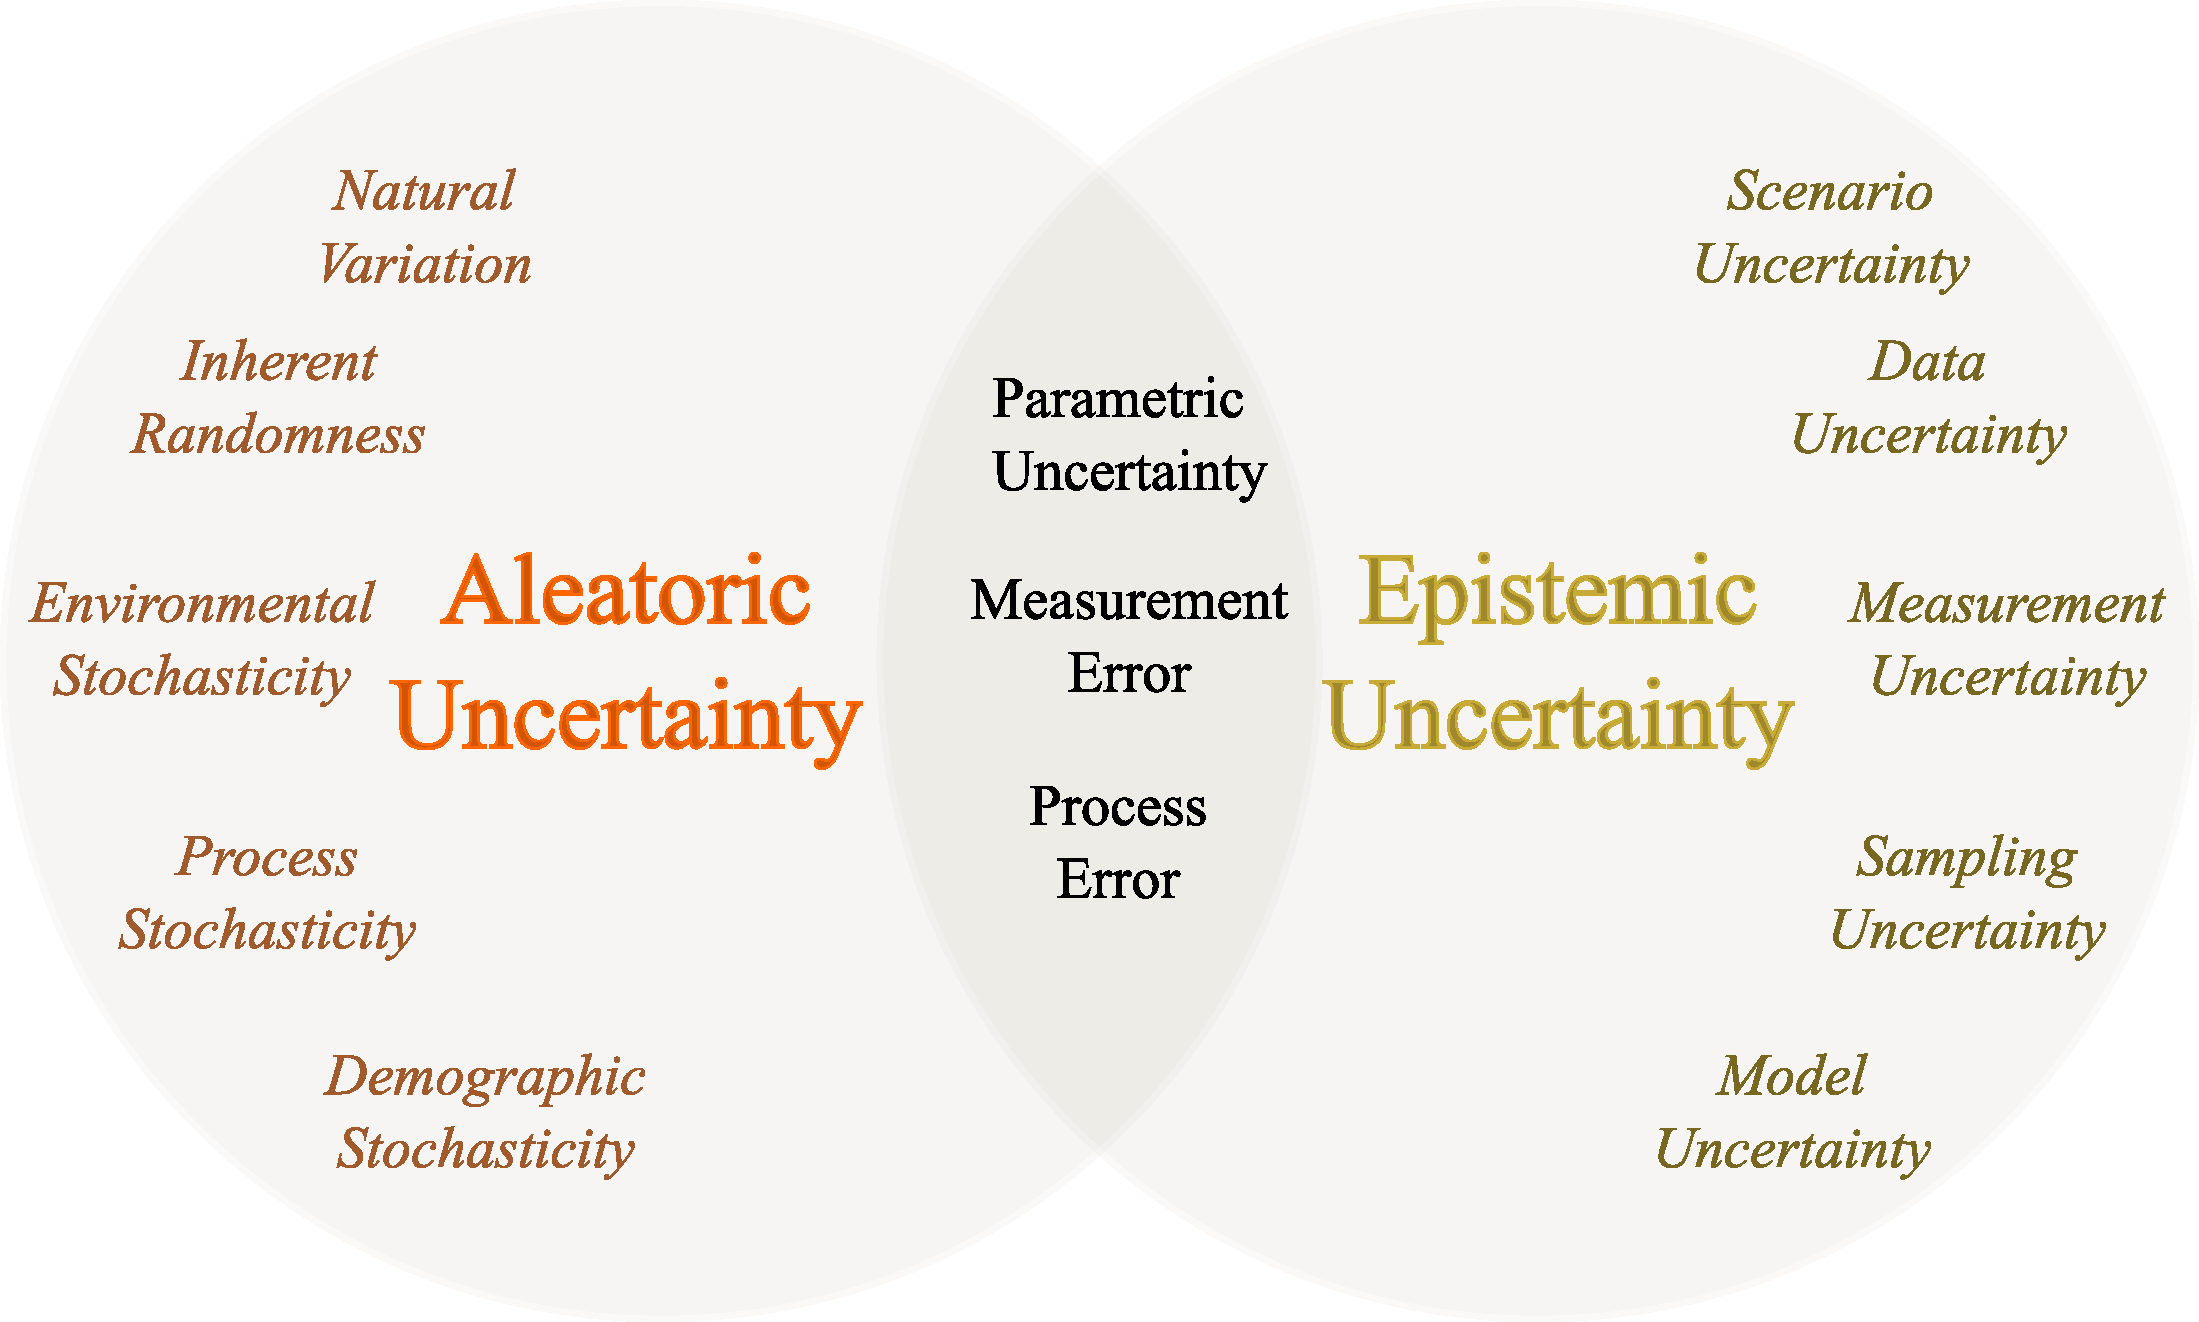
\includegraphics[scale=0.3]{figures/figure-uncertainty_classification.pdf}
\end{figure}
\end{frame}

%----------------------------------------------------------------------------
\begin{frame}
\frametitle{What about uncertainties in geotechnics}

    \begin{figure}
    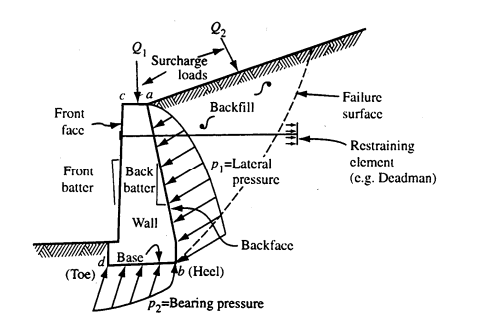
\includegraphics[scale=0.3]{figures/figure-retainingwall.png}    
    \hfill
    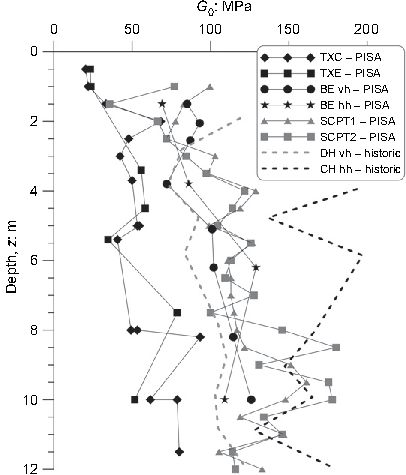
\includegraphics[scale=0.5]{figures/figure-UQtype2.pdf}
    \tiny\footcite{zdravkovic2020}
    \hfill
    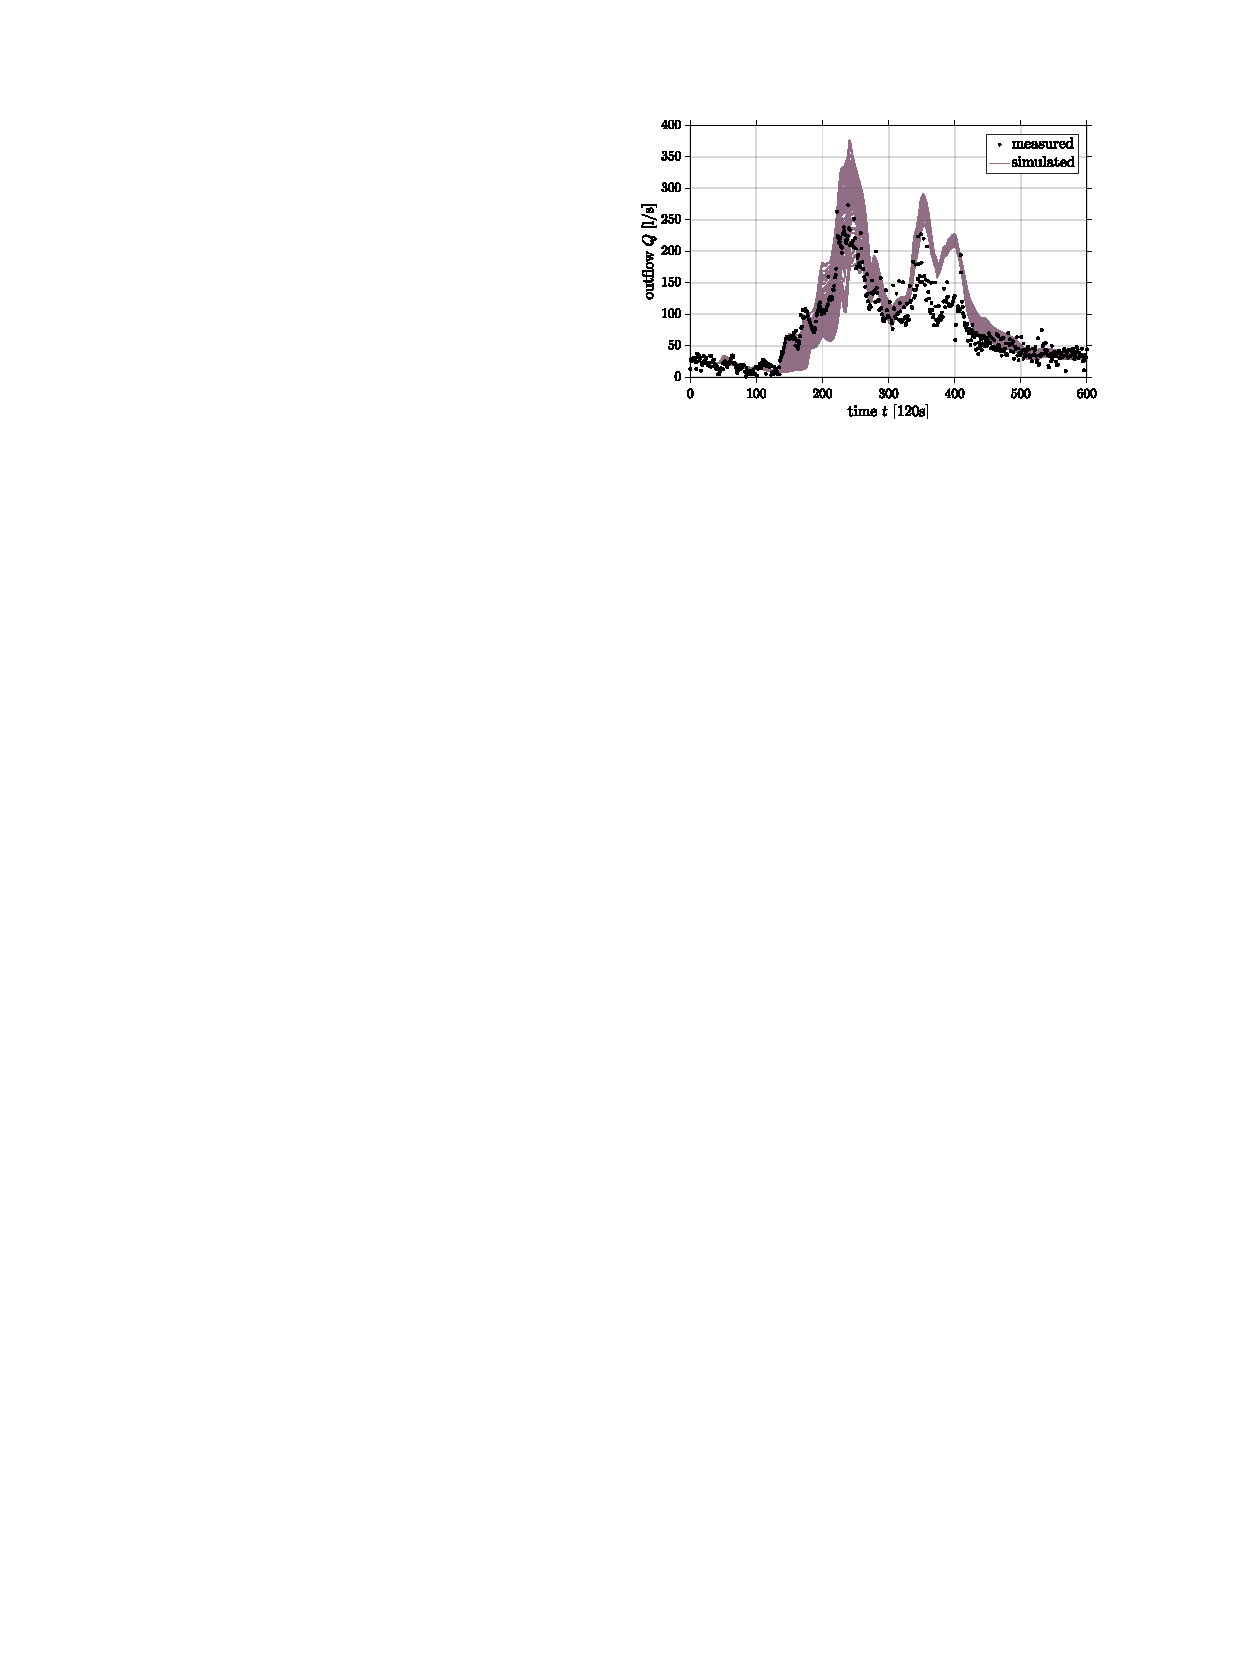
\includegraphics[scale=0.65]{figures/figure-UQtype3.pdf}
    \footfullcite{nagel2020}  
    \end{figure}
\end{frame}
